\section{Project Review}

	\subsection{Discussion}
	\begin{frame}[t]{Project Review}\framesubtitle{Parallel Computing Platform}
	\begin{columns}[T]
	\begin{column}{0.48\textwidth}
		\begin{itemize}
			\item OpenCL
			%Different supported versions for each manufacturer
			\item CUDA
			%Specifikt, men bedre til den specifikke
			\item Operating Systems
			%WindowsNoWork, manual library and platform linking
			%OpenCL Code cant runt, Our compiler runs fine
		\end{itemize}
	\end{column}
	\begin{column}{.48\textwidth}
      \begin{figure}
         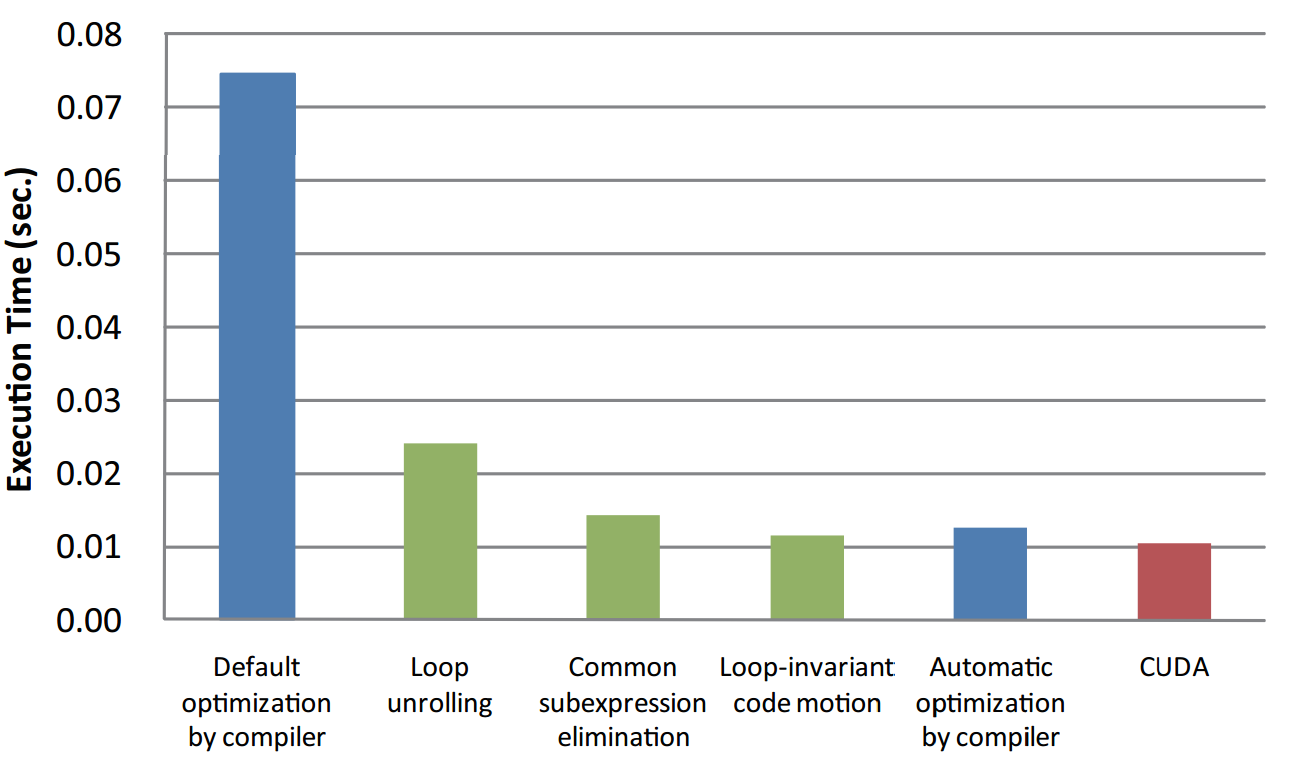
\includegraphics[width=1\textwidth]{images/opencloptimisation.png}
      \end{figure}
    \end{column}
    \end{columns}
	\end{frame}

	\begin{frame}[t]{Project Review}\framesubtitle{Seamless GPU Usage}
		\begin{itemize}
			\item User Control
			%Brugeren har 0 kontrol over fordeling
			\item Predefined Operations
			%Kun enkelte predefinerede operationer udregnes på GPU, og for disse er der intet alternatitv der tillader brug af CPU
			%Ingen functioner/loops
			\item Efficiency
			%I forhold til de steder hvor GPU udnyttes kontra andre steder den måske kunne udnyttes
		\end{itemize}
	\end{frame}

	\subsection{Conclusion}
	\begin{frame}[t]{Project Review}\framesubtitle{Conclusion}
	\begin{columns}[T]
	\begin{column}{0.48\textwidth}
		\begin{itemize}
		%Eventuelt starte med problemformulering/sprog kriterier?
			\item Seamless GPU utilisation
			 %+Read and writability
			\item Runtime Efficiency
			%GPU Improves performance, could be improved more however
			\item Cross Platform Solution vs. Single Platform Solution
			%Because we use a module design of our compiler, simply changing the code generation module could swap to Cuda/Specific platform targeting
			\begin{itemize}
				\item Broader range
				\item Generelisation reduces efficiency
			\end{itemize}
			%Laves eventuelt om til eget slide
			\item Development Process
			\begin{itemize}
				\item Iterative
				\item Realisations in Code Generation
				\item Not enough operators
			\end{itemize}
			%IterativUdvikling
			%Primær gains Når Code Gen noget, reworked tidligere fordi der er fundet yderligere ting der ønskes/nogle ting skulle ændres
			%Functions > Operators changes to Operators > Functions i forhold til matrice operationer
			%Hvorfor tænkte vi på Funcs > Operatorer i starten?
			%Explicit fordi * kan have flere betydninger i matrice verdenen - kernels gav problemer som funktioner
			%Modulær fordeling gavner også her
		\end{itemize}
	\end{column}
	\begin{column}{.48\textwidth}
      \begin{figure}
         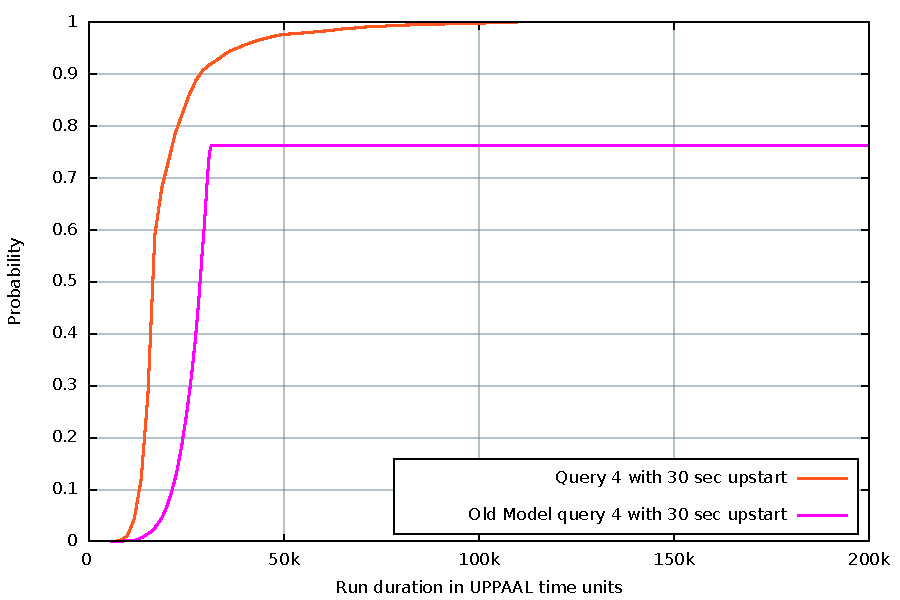
\includegraphics[width=1\textwidth]{images/graph.pdf}
      \end{figure}
    \end{column}
    \end{columns}
	\end{frame}

	\subsection{Future Works}
	\begin{frame}[t]{Project Review}\framesubtitle{Future Works}
	\begin{columns}[T]
	\begin{column}{0.48\textwidth}
		\begin{itemize}
			\item Code Analysis And User Control
			\begin{itemize}
				\item More user responsibility
				\item Can increase runtime efficiency
				\item Templates are not an effective solution
			\end{itemize}
			%Bedre fordeling af udregninger på platforme, både nativt og explicit har mulighed for at øge runtime efficiency i stor grad, muligheden for explicit gpu brug tillader desuden brugen flere steder end nativt, blot tradeoff er ansvar på bruger
			%Templates reducere effeciency
			\item Kernel Improvements
			%Bedre brug af memory, platform targeting virker yderligere her da Nvidia har anderledes architectur(Warps i thread hierarchy(thread>warp>ThreadBlock>Grid/Thread>WorkGroup>NDRange))
			%Possible improvements instead of Templates?(making functions available)
			%a+b+c er 2 kernels frem for 1
			\item Platform Targeting
			%Platform targeting øger performance på den specifikke platform
			%Bedre end en universel cross platform løsning
			%Kan i princippet targetes til hver enkelt GPU størrelse(meget arbejde) men eventuelt lave generationelle versioner(en der passer til ca. 500)?
		\end{itemize}
	\end{column}
	\begin{column}{.48\textwidth}
      \begin{figure}
         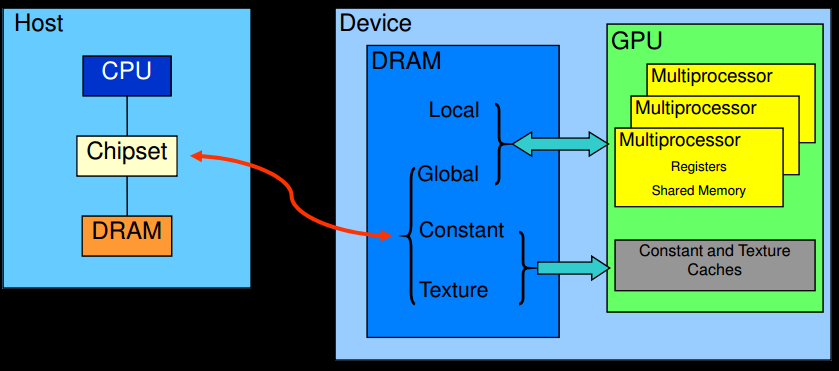
\includegraphics[width=1\textwidth]{images/GPUMemoryClear.png}
      \end{figure}
    \end{column}
    \end{columns}
	\end{frame}

	\begin{frame}[t]{Project Review}\framesubtitle{Future Works}
	\begin{columns}[T]
	\begin{column}{0.48\textwidth}
		\begin{itemize}
			\item Code Analysis And User Control
			%Bedre fordeling af udregninger på platforme, både nativt og explicit har mulighed for at øge runtime efficiency i stor grad, muligheden for explicit gpu brug tillader desuden brugen flere steder end nativt, blot tradeoff er ansvar på bruger
			%Templates reducere effeciency
			\item Kernel Improvements
			\begin{itemize}
				\item Memory handling
				\item Nvidia different memory hierarchy, Warps
				\item Templates
			\end{itemize}
			%Bedre brug af memory, platform targeting virker yderligere her da Nvidia har anderledes architectur(Warps i thread hierarchy(thread>warp>ThreadBlock>Grid/Thread>WorkGroup>NDRange))
			%Possible improvements instead of Templates?(making functions available)
			%a+b+c er 2 kernels frem for 1
			\item Platform Targeting
			%Platform targeting øger performance på den specifikke platform
			%Bedre end en universel cross platform løsning
			%Kan i princippet targetes til hver enkelt GPU størrelse(meget arbejde) men eventuelt lave generationelle versioner(en der passer til ca. 500)?
		\end{itemize}
	\end{column}
	\begin{column}{.48\textwidth}
      \begin{figure}
         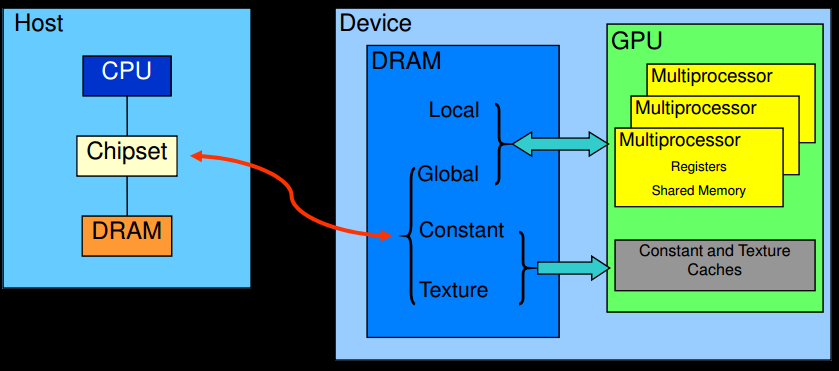
\includegraphics[width=1\textwidth]{images/GPUMemoryClear.png}
      \end{figure}
    \end{column}
    \end{columns}
	\end{frame}

	\begin{frame}[t]{Project Review}\framesubtitle{Future Works}
	\begin{columns}[T]
	\begin{column}{0.48\textwidth}
		\begin{itemize}
			\item Code Analysis And User Control
			%Bedre fordeling af udregninger på platforme, både nativt og explicit har mulighed for at øge runtime efficiency i stor grad, muligheden for explicit gpu brug tillader desuden brugen flere steder end nativt, blot tradeoff er ansvar på bruger
			%Templates reducere effeciency
			\item Kernel Improvements
			%Bedre brug af memory, platform targeting virker yderligere her da Nvidia har anderledes architectur(Warps i thread hierarchy(thread>warp>ThreadBlock>Grid/Thread>WorkGroup>NDRange))
			%Possible improvements instead of Templates?(making functions available)
			%a+b+c er 2 kernels frem for 1
			\item Platform Targeting
			\begin{itemize}
				\item More efficient resource usage
				\item Specifications specialisation
			\end{itemize}
			%Platform targeting øger performance på den specifikke platform
			%Bedre end en universel cross platform løsning
			%Kan i princippet targetes til hver enkelt GPU størrelse(meget arbejde) men eventuelt lave generationelle versioner(en der passer til ca. 500)?
		\end{itemize}
	\end{column}
	\begin{column}{.48\textwidth}
      \begin{figure}
         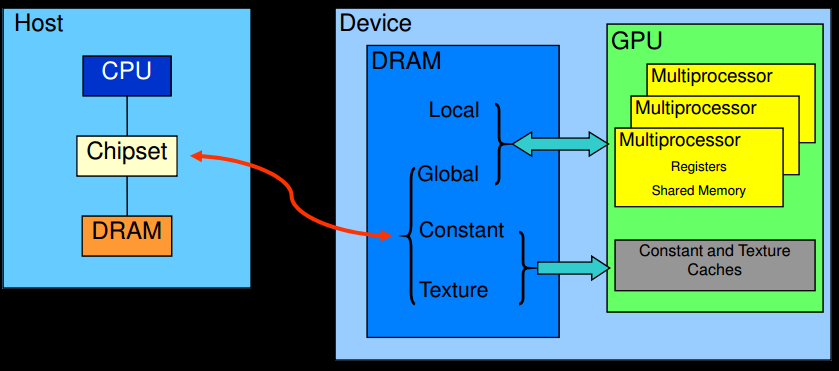
\includegraphics[width=1\textwidth]{images/GPUMemoryClear.png}
      \end{figure}
    \end{column}
    \end{columns}
	\end{frame}